\section{MongoDB}
\subsection{Einleitung}
Schemalose NoSQL Datenbanksysteme werden in der heutigen Zeit immer öfters verwendet, dank ihrer Flexibilität, Geschwindigkeit und Verlässlichkeit. MongoDB ist ein schemaloses Datenbanksystem, die auf Dokumentenspeicherung basiert. Diese Dokumente von MongoDB speichern die Daten in einem JSON ähnlichen, nämlich BSON (Binary JSON), was speziell für MongoDB erstellt wurde, Format. Hierbei spielt es keine Rolle, wie die Daten aufgebaut sind, die in das Dokument eingetragen werden. Dokumente in MongoDB werden in Collections gespeichert. Jede Collection fügt einem Dokument eine eindeutige ID zu.  Die Dateigröße für Dokumente beträgt maximal 16MB. Eine Ansammlung von Collections stellt die Datenbank dar.
Der Aufbau von einer Datenbank in MongoDB sieht wie folgt aus:
\\
\\
\begin{minipage}{\textwidth}
    \centering
    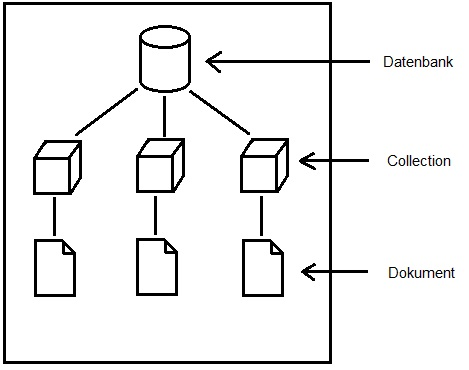
\includegraphics[scale=0.9]{images/Datenmodell_Mongo.jpg}
    \captionof{figure}{Datenbankstruktur von MongoDB}
    \label{fig:ver}
\end{minipage}
\\
Die Collection kann man wie eine Tabelle in einer relationalen Datenbank ansehen und die Dokumente sind die jeweiligen Reihen, also die konkrete Dateneintragungen in die Tabelle.
\subsection{Geschichte}
MongoDB wurde von Dwight Merriman, Eliot Horowitz und seinem Team erstellt. Doch dies nicht auf direktem Wege. 2007 plante das MongoDB Team ein Onlineservice für Web-Anwendungen. Dieser Service sollte die Möglichkeit bieten, eine Web-Anwendung zu entwickeln, zu hosten und zu skalieren. Aufgrund von einem nicht geeigneten Datenbanksystem entschloss sich das Team ein eigenes Datenbanksystem zu erstellen und zu nutzen. Diese hatte noch keinen Namen, da dieses System speziell für den Service des Teams erstellt wurde. Im Jahre 2008 wurde dann das Datenbanksystem fertiggestellt. 2009 entschloss sich das Team, dieses Datenbanksystem, was sie erstellt haben, als Open Source Produkt freizugeben. Dieses System wurde als MongoDB veröffentlicht. März 2010 kam die erste Version von MongoDB heraus, die man in einem größeren Umfang verwenden kann. Über die Jahre wurde MongoDB von dem Team weiterentwickelt und ist zurzeit mit der Version 3.2 veröffentlicht. 
\subsubsection{Philosophie}
Die Philosophie von MongoDB ist im Vergleich zu den meisten anderen etwas unterschiedlich. Denn das Team von MongoDB hat sich dazu entschieden, dass MongoDB nicht die Lösung für jedes Problem sein soll. MongoDB soll eine Lösung für Analytische Probleme und komplexe Datenstrukturen. Zudem liegt der Fokus auf die Nutzung von Dokumenten, nicht auf Zeilen. Das MongoDB Team wollte ein Datenbanksystem was sehr schnell, gut skalierbar und einfach anzuwenden ist.
\subsection{Anwendungsfälle}
MongoDB wird von verschiedenen Unternehmen zu verschiedensten Anwendungen und Aufgaben verwendet.
MTV verwendet MongoDB als Haupt-repository für das MTV-Network.
SourceForge verwendet MongoDB als Back-End Speicher.
Bit.ly verwendet MongoDB, um den Verlauf von Nutzern zu speichern.
New York Times verwendet MongoDB  für eine Foto-Abgabe.
\subsection{Einrichtung}
MongoDB wird für alle Betriebssysteme angeboten und ist derzeit in der Version 3.2 erhältlich. Dadurch lässt sich MongoDB auf Ubuntu 12.04+, Windows Server 2008+ und Mac OS X 10.7+ installieren und verwenden. 
Um MongoDB auf einem Linux Ubuntu Server zu installieren, muss man folgende Schritte befolgen:
\\
\\
1. Importierung von dem public key durch das package management System.
\\
2. Ein Listen-Datei für MongoDB erstellen.
\\
3. Lokale Dateien aktualisieren.
\\
4. Installation von MongoDB Paket.
\\
\\
Um MongoDB auf einem Windows Server zu installieren, muss man wie folgt vorgehen:
\\
\\
1. Bestimmen, welchen Build von MongoDB benötigt wird.
\\
2. MongoDB für Windows runterladen.
\\
3. Installation von MongoDB via Asministrator Kommandozeile.
\\
\\
Um MongoDB auf einem Mac OS System zu installieren, sind folgende Schritte notwendig:
\\
\\
1. Binäre Dateien von der benötigten MongoDB Version runterladen.
\\
2. Heruntergeladene Dateien extrahieren.
\\
3. Extrahierte Dateien in das Zielverzeichnis kopieren.
\\
4. Pfad von MongoDB sicherstellen.
\\
\\
Alle Vorgehensweisen für die Installation von MongoDB verwenden eine Kommandozeile.
%\subsubsection{Indexierung}
\subsubsection{Referenzierung}
Die Referenzierung von MongoDB unterscheidet sich von der Referenzierung von den relationalen Datenbanken. Eine Möglichkeit der Referenzierung in MongoDB wäre die Verschachtlung, also ein Dokument in einem Dokumenten schreiben. Damit kann man die Referenz auf ein anderes Objekt direkt erkennen, was auch für das System einfacher ist, an diese Daten zu gelangen. Das Problem hierbei kann aber eine zu starke Verschachtelungsstruktur sein, was auf Kosten der Übersichtlichkeit geht, zusätzlich wird für ein Dokument mehr Platz gebraucht, da in einem Dokument ein weiteres existiert. Die zweite Möglichkeit für eine Referenzierung, wäre der Verweis auf das jeweilige Dokument. Das verbessert die Übersicht und man kann erkennen, voraus die Daten herkommen. Ein Problem was MongoDB mit sich bringt, ist, dass es keine Direktreferenzierung gibt. In der Relationalen Datenbank kann man mit dem JOIN Befehl die Referenz zu einem anderen Datensatz in Bezug auf einen anderen Datensatz direkt ansprechen und anzeigen lassen. Dies kann MongoDB nicht. Um dies zu ermöglichen, muss man das in einer eigenen Applikation programmieren. 
\subsubsection{Replikation}
Eine Replikation bei MongoDB ist die Kopie von Daten auf weiteren Servern. Dies nennt man replica set. Ein replica set umfasst Server mit derselben Funktionalität und Dient zur Stabilisierung der Aufgabe des jeweiligen replica sets. Die MongoDB Website empfiehlt das Verwenden von drei Servern pro replica set, um somit die Ausfallrate gering zu halten. Die Daten in einem replica set sind auf allen Servern identisch. MongoDB verwendet das Master-Slave System für die Replikation von Daten innerhalb des replica sets. In dem replica set gibt es genau einen Primary und beliebig viele Secondary Server und ggf. einen Arbiter. Datenänderungen wie z.B. Schreiboperationen werden auf dem Primary Server in dem replica set durchgeführt. Nachdem die Operation erfolgreich beendet wurde, übernehmen die Secondary Server die Änderung von dem Primary Server. Sollte der Primary Server ausfallen, so wählen die Secondary Server einen neuen Primary Server aus. Man ist in der Lage, in dem replica set einen Arbiter hinzuzufügen. Ein Arbiter besitzt nicht die Daten, die in dem replica set verteilt werden. Der Arbiter dient lediglich dazu, nur bei einer Abstimmung eine Stimme abzugeben, damit eventuelle Probleme bei einer Abstimmung vermieden werden können. Ein Arbiter selber kann nicht zu einem Primary oder Secondary Server ernannt werden.
\\
\\
\begin{minipage}{\textwidth}
    \centering
    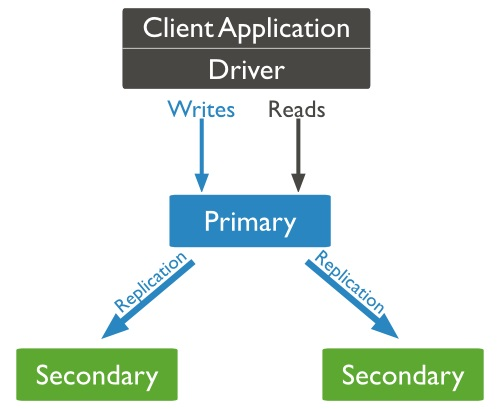
\includegraphics[scale=0.9]{images/replica-set-read-write-operations-primary.jpg}
    \captionof{figure}{Replikationsaufbau von MongoDB}
    \label{fig:ver}
\end{minipage}
\subsubsection{Cluster Sharding}
Ein sharded Cluster bei MongoDB ist eine Methode, um Daten auf unterschiedlichen Servern zu speichern und dann diese schnell aufzurufen. Ein sharded cluster besteht aus drei Komponenten: Den Config Server, den Query Server und Shards. Um ein sharded cluster einzurichten, braucht man mindestens einen Config Server, einen Query Server und 2 Shards. Dies sieht dann wie folgt aus:
\\
\\
\begin{minipage}{\textwidth}
    \centering
    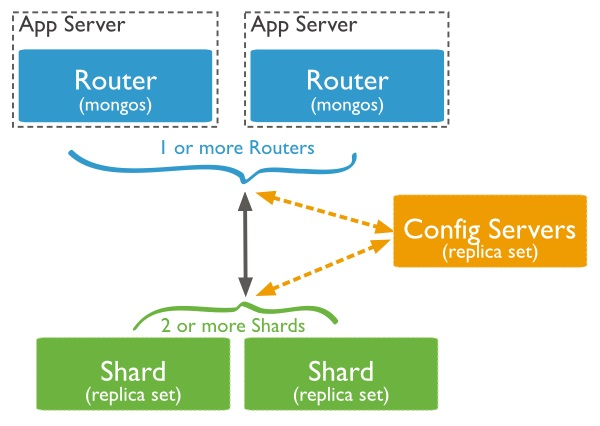
\includegraphics[scale=1.0]{images/sharded-cluster-production-architecture.jpg}
    \captionof{figure}{Aufbau vom Cluster Sharding in MongoDB}
    \label{fig:ver}
\end{minipage}
\\
\\
Config Server: Der Config Server in einem sharded Cluster beinhaltet die Metadaten für dieses. Diese Metadaten beinhalten die Informationen zu der Organisation und die Zustände der jeweiligen Komponenten in dem sharded Cluster.  Ein Config Server ist in einem replica set. Ein replica set verbessert die Konsistenz über die verschiedenen Config Server. Zusätzlich kann man danke dem replica set mehr als 3 Config Server nutzen.
Query Server (Router): Mit dem Query Server ist man in der Lage, Daten auf den verschiedenen Shards zu schreiben und zu Lesen. Dies vollbringt er mit den Metadaten, die der Query Server von dem Config Server bekommt. Der Query Server ist die einzige Schnittstelle in dem sharded Cluster, womit man auf die Daten durch Anwendungen zugreifen kann. 
\\
\\
\begin{minipage}{\textwidth}
    \centering
    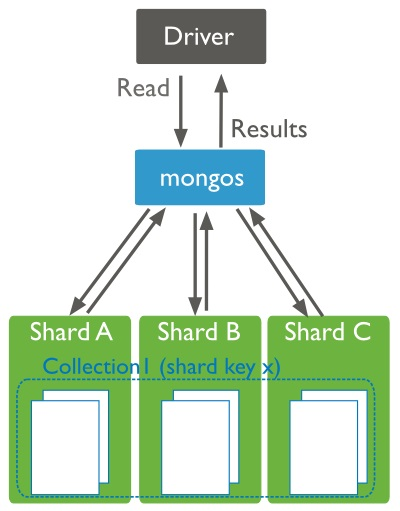
\includegraphics[scale=0.9]{images/sharded-cluster-scatter-gather-query.jpg}
    \captionof{figure}{Datenverteilung von dem Query Server}
    \label{fig:ver}
\end{minipage}
\\
\\
Shard: Bei einer Shard handelt es sich um einen Teil der Gesamtdatenbank. Die Daten, die in die Datenbank eingetragen werden, werden nach den Metadaten des Configservers analysiert und dann durch den Query Server auf das jeweilige Shard gespeichert. Zum Beispiel: Eine 3 Shard Datenbank beinhaltet Daten von Personen in einem Unternehmen. Auf Shard 1 werden alle Mitarbeiter gespeichert, die im Nachnamen mit dem Buchstaben A bis H anfangen. Shard 2 hat den Nachnamen von I bis Q und Shard 3 R bis Z. Dadurch, dass die Daten aufgeteilt und auf unterschiedlichen Shards gespeichert werden, ist man in der Lage schneller an die gewünschten Informationen zu kommen. Shards können sich in einem replica set befinden. Dieses dient für Redundanz  und hohe Verfügbarkeit der Daten.
\subsection{Verwendung}
Um mit MongoDB Daten einzufügen oder auszulesen, sind verschiedene CRUD-Operationen notwendig, wie bei einer relationellen Datenbank. Diese Operationen ähneln wie JavaScript Anweisungen und sind daher leicht anzuwenden. Die wichtigsten Befehle zur Verwendung von MongoDB sind in Tabelle 2.1 zu entnehmen.
\\
\\
\begin{table}[h]
\centering
\begin{tabular}{p{7cm}|p{7cm}|c|c|}
\hline 
Befehl & Funktion \\ 
\hline 
Use <Datenbankname> & Setzt die Datenbank zu den benutzten Namen \\ 
\hline 
db.createCollection(„Name“,{capped : true, size : <byte>, max : <anzahl> }) & Legt eine Collection mit dem angegebenen Namen \\ 
\hline 
db.<name>.insert({Name: „Thomas“, Alter: 25, …})  & Legt ein Dokument in der Collection <name> ab \\ 
\hline 
db.<name>.save({Name: „Thomas“, Alter: 22}) & Einfache Veränderung eines Dokumentes mit dem Namen “Thomas” \\ 
\hline 
db.<name>.update({Name: „Thomas“}, {Name: „Franz“ , Alter: 24}) & Veränderung eines Dokumentes mit dem Namen „Thomas“ \\ 
\hline 
db.<name>.find() & Zeigt alle Dokumente in der Collection <name> \\ 
\hline 
db.<name>.count({Name: „Franz“}) & Zählt alle Dokumente, die den Namen “Franz” beinhalten \\ 
\hline 
db.<name>.remove({Name: “Franz”}) & Löscht alle Dokumente mit dem Namen “Franz” \\ 
\hline 
db.<name>.drop() & Die Collection löschen \\ 
\hline 
\end{tabular}
\caption{Befehlsliste für MongoDB}
\end{table} 
\\
Beim Arbeiten von MongoDB sollte stets geachtet werden, dass man auf der richtigen Datenbank arbeitet und dass die Dokumente in die richtige Collections eingetragen werden. Zudem sollte man auf Groß-  und Kleinschreibung achten, da MongoDB Case-Sensitive ist. 
\subsection{Grenzen}
MongoDB besitzt in mehrere Bereiche Limitationen, die die Performance und das Nutzen von MongoDB einschränken. 
\begin{itemize}
\item 32bit Version von MongoDB kann nur eine Datenbank einrichten, die maximal 2 GB groß sein kann. Dieses Problem kann behoben werden, indem man die 64bit Version von MongoDB verwendet. Zudem wird die 32bit Version von MongoDB nicht mehr seit der 3.0 Version unterstützt.
\item BSON Dokumente können maximal 16MB groß sein, was aber in Vergleich zu anderen Datenbanksystemen sehr groß ist.
\item Indexe in MongoDB können nicht größer als 1024 Byte sein. Zudem kann eine Collection maximal 64 Indexe besitzen. Auch der Name des Indexes ist auf 128 Byte begrenzt. Diese Limitationen sollten bei einer gut aufgebauten Datenbank nicht erreicht werden.
\item Sobald eine Collection mit einer Grenze eingestellt wurde, kann diese nicht erweitert werden. Das maximum was man bei der Grenzeinstellung vornehmen kann ist 232 Dokumente. Man ist aber auch in der Lage, diese Grenze auszustellen. Sollte die Grenze erreicht werden, kann man nur mit einer neuen Collection mit einer größeren oder keiner Grenze das Problem beheben.
\item Das Sharding sollte wenn möglich so früh wie möglich eingeführt werden, da sonst die Performance von MongoDB stark beeinträchtigt wird, da die Server die Daten auf den unterschiedlichen Shards verteilen muss. Zudem sollte auch geachtet werden, das die Datenbank nicht über 256 GB groß ist, da MongoDB bei einer Größe von 256 GB das Sharding nicht mehr erlaubt.
\item Die Daten die bei MongoDB versendet werden sind nicht verschlüsselt.
Bei Lese und Schreibvorgänge bei der MongoDB muss man auf Groß- und Kleinschreibung achten, da MongoDB Case-Sensitive ist.
\item MongoDB besitzt keine JOIN-Operation. Man muss diese durch verschachtelte Dokumente oder auf einen verweis auf das jeweilige Dokument machen.
\end{itemize}